
\documentclass{article}

\usepackage{amsthm}
\usepackage{amsfonts}
\usepackage{amsmath}
\usepackage{amssymb}
\usepackage{fullpage}
\usepackage{graphicx}

\usepackage{tikz}
\usepackage[usenames]{color}
\usepackage{hyperref}
  \hypersetup{
    colorlinks = true,
    urlcolor = blue,       % color of external links using \href
    linkcolor= blue,       % color of internal links 
    citecolor= blue,       % color of links to bibliography
    filecolor= blue,        % color of file links
    }
    
\usepackage{listings}

\definecolor{dkgreen}{rgb}{0,0.6,0}
\definecolor{gray}{rgb}{0.5,0.5,0.5}
\definecolor{mauve}{rgb}{0.58,0,0.82}

\lstset{frame=tb,
  language=haskell,
  aboveskip=3mm,
  belowskip=3mm,
  showstringspaces=false,
  columns=flexible,
  basicstyle={\small\ttfamily},
  numbers=none,
  numberstyle=\tiny\color{gray},
  keywordstyle=\color{blue},
  commentstyle=\color{dkgreen},
  stringstyle=\color{mauve},
  breaklines=true,
  breakatwhitespace=true,
  tabsize=3
}

\theoremstyle{theorem} 
   \newtheorem{theorem}{Theorem}[section]
   \newtheorem{corollary}[theorem]{Corollary}
   \newtheorem{lemma}[theorem]{Lemma}
   \newtheorem{proposition}[theorem]{Proposition}
\theoremstyle{definition}
   \newtheorem{definition}[theorem]{Definition}
   \newtheorem{example}[theorem]{Example}
\theoremstyle{remark}    
  \newtheorem{remark}[theorem]{Remark}


\title{CPSC-402 Report\\Compiler Construction}
\author{Your Name  \\ Chapman University}

\date{\today}

\begin{document}

\maketitle

\begin{abstract}
Short  summary of purpose and content.  
\end{abstract}

\tableofcontents

\section{Introduction}\label{intro}

Replace this entire Section~\ref{intro} with your own short introduction. 

\subsection{General Remarks}

First you need to \href{https://www.latex-project.org/get/}{download and install} LaTeX.\footnote{Links are typeset in blue, but you can change the layout and color of the links if you locate the  \texttt{hypersetup} command.}
%
For quick experimentation, you can use an online editor such as \href{https://www.overleaf.com/learn}{Overleaf}. But to grade the report I will used the time-stamped pdf-files in your git repository.  

 
\medskip\noindent
LaTeX is a markup language (as is, for example, HTML). The source code is in a \verb+.tex+ file and needs to be compiled for viewing, usually to \verb+.pdf+.


\medskip\noindent
If you want to change the default layout, you need to type commands. For example, \verb+\medskip+ inserts a medium vertical space and \verb+\noindent+ starts a paragraph without indentation.
 
\medskip\noindent
Mathematics is typeset between double dollars, for example $$x+y=y+x.$$


\subsection{LaTeX Resources}

I start a new subsection, so that you can see how it appears in the table of contents.

\subsubsection{Subsubsections}

Sometimes it is good to have subsubsections.

\subsubsection{Itemize and enumerate}

\begin{itemize}
\item This is how you itemize in LaTeX.
\item I think a good way to learn LaTeX is by starting from this template file and build it up step by step. Often stackoverflow will answer your questions. But here are a few resources:
  \begin{enumerate}
  \item \href{https://www.overleaf.com/learn/latex/Learn_LaTeX_in_30_minutes}{Learn LaTeX in 30 minutes}
  \item \href{https://www.latex-project.org/}{LaTeX – A document preparation system}\end{enumerate}
\end{itemize}

\subsubsection{Typesetting Code}

A typical project will involve code. For the example below I took the LaTeX code from \href{https://stackoverflow.com/a/3175141/4600290}{stackoverflow} and the Haskell code from \href{https://hackmd.io/@alexhkurz/HylLKujCP}{my tutorial}.

\begin{lstlisting}
-- run the transition function on a word and a state
run :: (State -> Char -> State) -> State -> [Char] -> State
run delta q [] = q
run delta q (c:cs) = run delta (delta q c) cs 
\end{lstlisting}
%
Short snippets such as \texttt{run :: (State -> Char -> State) -> State -> [Char] -> State} can also be directly fitted into text. There are several ways of doing this, for example, \verb@run :: (State -> Char -> State) -> State -> [Char] -> State@ is slightly different in terms of spaces and linebreaking (and can lead to layout that is better avoided), as is
\begin{verbatim}run :: (State -> Char -> State) -> State -> [Char] -> State\end{verbatim}

\noindent
For more on the topic see \href{https://www.overleaf.com/latex/examples/code-presentations-example-different-ways-shown-in-beamer-metropolis/tsxpnyjbhbds}{Code-Presentations Example}.

\medskip\noindent
Generally speaking,  the methods for displaying code discussed above work well only for short listings of code. For entire programs, it is better to have external links to, for example, Github or \href{https://replit.com/@alexhkurz/automata01#main.hs}{Replit} (click on the "Run" button and/or the ``Code" tab).

\subsubsection{Including Graphics}

By way of example, I include here a screenshot from the book \cite{Hopcroft}.

\includegraphics{automaton-example.png}

\noindent
You can use the same technique to include any handwritten drawings.

\subsubsection{More Mathematics}

We have already seen $x+y=y+x$ as an example of inline maths. We can also typeset mathematics in display mode, for example
$$\frac x y =\frac{xy}{y^2},$$

\noindent
Here is an example of equational reasoning that spans several lines:
\begin{align*}
{\rm fib}(3)
& = {\rm fib}(1) +{\rm fib}(2)  & {\rm fib}(n+2) = {\rm fib}(n)  + {\rm fib}(n+1) \\
& = {\rm fib}(1) +{\rm fib}(0)  + {\rm fib}(1) & {\rm fib}(n+2) = {\rm fib}(n)  + {\rm fib}(n+1) \\
& = 1 + 0  +1 & {\rm fib}(0) = 0,   {\rm fib}(1) = 1\\
& = 2 & {\rm arithmetic}
\end{align*}

\subsubsection{Definitons, Examples, Theorems, Etc}

\begin{definition} 
This is a definition.
\end{definition}

\begin{example}
This is an example.
\end{example}

\begin{proposition}
This is a proposition.
\end{proposition}

\begin{theorem}
This is a theorem.
\end{theorem}

\noindent You can also create your own environment, eg if you want to have Question, Notation, Conjecture, etc.

\subsection{Plagiarism}

To avoid plagiarism, make sure that, in addition to my course notes, you also cite all the external sources you use. Make sure you cite your references throughout your text, not only at the end.

\section{Homework}\label{homework}

This section will contain your solutions to homework. 

\subsection{Week 1}

\textbf{Exercise 2.2.4} Give DFA's accepting the following languagues over the lpahbet {0, 1}:\\
 
 a) The set of all strings ending in 000\\
 b)The set of all strings with three consecutive 0's(net neccarilt at the end).\\
 c)  The set of strings with 011 as a substring
 
 \includegraphics{IMG-0493.jpg}
 
 
\subsection{Week 2}

\subsection{Week 3}


\subsubsection{3.2.4}

Convert the following regular expressions to NFAs.
\\

01*:
\begin{center}
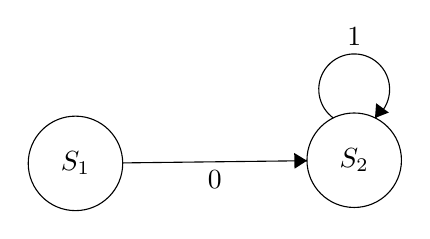
\begin{tikzpicture}[scale=0.2]
\tikzstyle{every node}+=[inner sep=0pt]
\draw [black] (3.2,-9.2) circle (3);
\draw (3.2,-9.2) node {$S_1$};
\draw [black] (20.9,-9) circle (3);
\draw (20.9,-9) node {$S_2$};
\draw [black] (6.2,-9.17) -- (17.9,-9.03);
\fill [black] (17.9,-9.03) -- (17.09,-8.54) -- (17.11,-9.54);
\draw (12.05,-9.61) node [below] {$0$};
\draw [black] (19.577,-6.32) arc (234:-54:2.25);
\draw (20.9,-1.75) node [above] {$1$};
\fill [black] (22.22,-6.32) -- (23.1,-5.97) -- (22.29,-5.38);
\end{tikzpicture}
\end{center}

(0 + 1)01:
\begin{center}
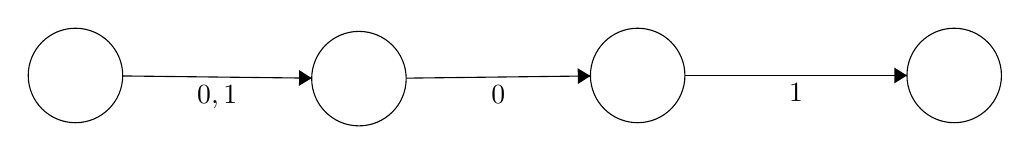
\begin{tikzpicture}[scale=0.2]
\tikzstyle{every node}+=[inner sep=0pt]
\draw [black] (3.3,-3.2) circle (3);
\draw [black] (21.3,-3.4) circle (3);
\draw [black] (39,-3.2) circle (3);
\draw [black] (59.1,-3.2) circle (3);
\draw [black] (6.3,-3.23) -- (18.3,-3.37);
\fill [black] (18.3,-3.37) -- (17.51,-2.86) -- (17.49,-3.86);
\draw (12.3,-3.82) node [below] {$0,1$};
\draw [black] (24.3,-3.37) -- (36,-3.23);
\fill [black] (36,-3.23) -- (35.19,-2.74) -- (35.21,-3.74);
\draw (30.15,-3.81) node [below] {$0$};
\draw [black] (42,-3.2) -- (56.1,-3.2);
\fill [black] (56.1,-3.2) -- (55.3,-2.7) -- (55.3,-3.7);
\draw (49.05,-3.7) node [below] {$1$};
\end{tikzpicture}
\end{center}


00(0 + 1)*:
\begin{center}
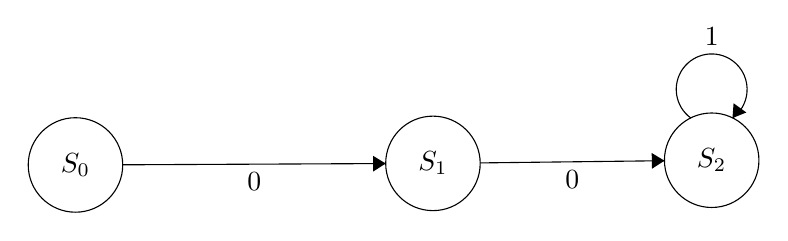
\begin{tikzpicture}[scale=0.2]
\tikzstyle{every node}+=[inner sep=0pt]
\draw [black] (25.9,-9.2) circle (3);
\draw (25.9,-9.2) node {$S_1$};
\draw [black] (43.6,-9) circle (3);
\draw (43.6,-9) node {$S_2$};
\draw [black] (3.2,-9.3) circle (3);
\draw (3.2,-9.3) node {$S_0$};
\draw [black] (28.9,-9.17) -- (40.6,-9.03);
\fill [black] (40.6,-9.03) -- (39.79,-8.54) -- (39.81,-9.54);
\draw (34.75,-9.61) node [below] {$0$};
\draw [black] (42.277,-6.32) arc (234:-54:2.25);
\draw (43.6,-1.75) node [above] {$1$};
\fill [black] (44.92,-6.32) -- (45.8,-5.97) -- (44.99,-5.38);
\draw [black] (6.2,-9.29) -- (22.9,-9.21);
\fill [black] (22.9,-9.21) -- (22.1,-8.72) -- (22.1,-9.72);
\draw (14.55,-9.75) node [below] {$0$};
\end{tikzpicture}
\end{center}





\ldots

\section{Project}

The project will be to compile code from a programming language of your choice to assembly and to explain the assembly code and compilation process using the knowledge your learned in this course. 


\medskip\noindent
Pro tips:
\begin{itemize}
\item Choose a compiled (not interpreted) programming language.
\item Choose a language that you find interesting anyway.
\item Start early.
\item Come to office hours. I have not run this part of the course before and I am really interested what you will find.
\end{itemize}
 
\section{Conclusions}\label{conclusions}

(approx 400 words)

In the conclusion, I want a critical reflection on the content of the course. Step back from the technical details. How does the course fit into the wider world of programming languages and software engineering?

\begin{thebibliography}{99}
\bibitem[HMU]{Hopcroft}
	John E. Hopcroft, Rajeev Motwani, Jeffrey D. Ullman:
\href{http://ce.sharif.edu/courses/94-95/1/ce414-2/resources/root/Text%20Books/Automata/John%20E.%20Hopcroft,%20Rajeev%20Motwani,%20Jeffrey%20D.%20Ullman-Introduction%20to%20Automata%20Theory,%20Languages,%20and%20Computations-Prentice%20Hall%20(2006).pdf}{Introduction to automata theory, languages, and computation,} 3rd Edition. Pearson international edition, Addison-Wesley 2007

\end{thebibliography}

\end{document}
